
\subsection{Hardware Demonstration of Morphology-Coordinated Execution}
\label{sec:hardware}
The simulation study examines the feasible-space benefit of joint morphology planning and the behavior of rolling trajectory transitions. We next demonstrate the corresponding morphology-coordination principle on the physical aerial continuum platform. The task connects passage traversal, target approach, object handling, and return flight in a shared scene, providing a physical counterpart to the confined-passage and terminal-reaching scenarios.

\begin{figure*}[!t]
\centering
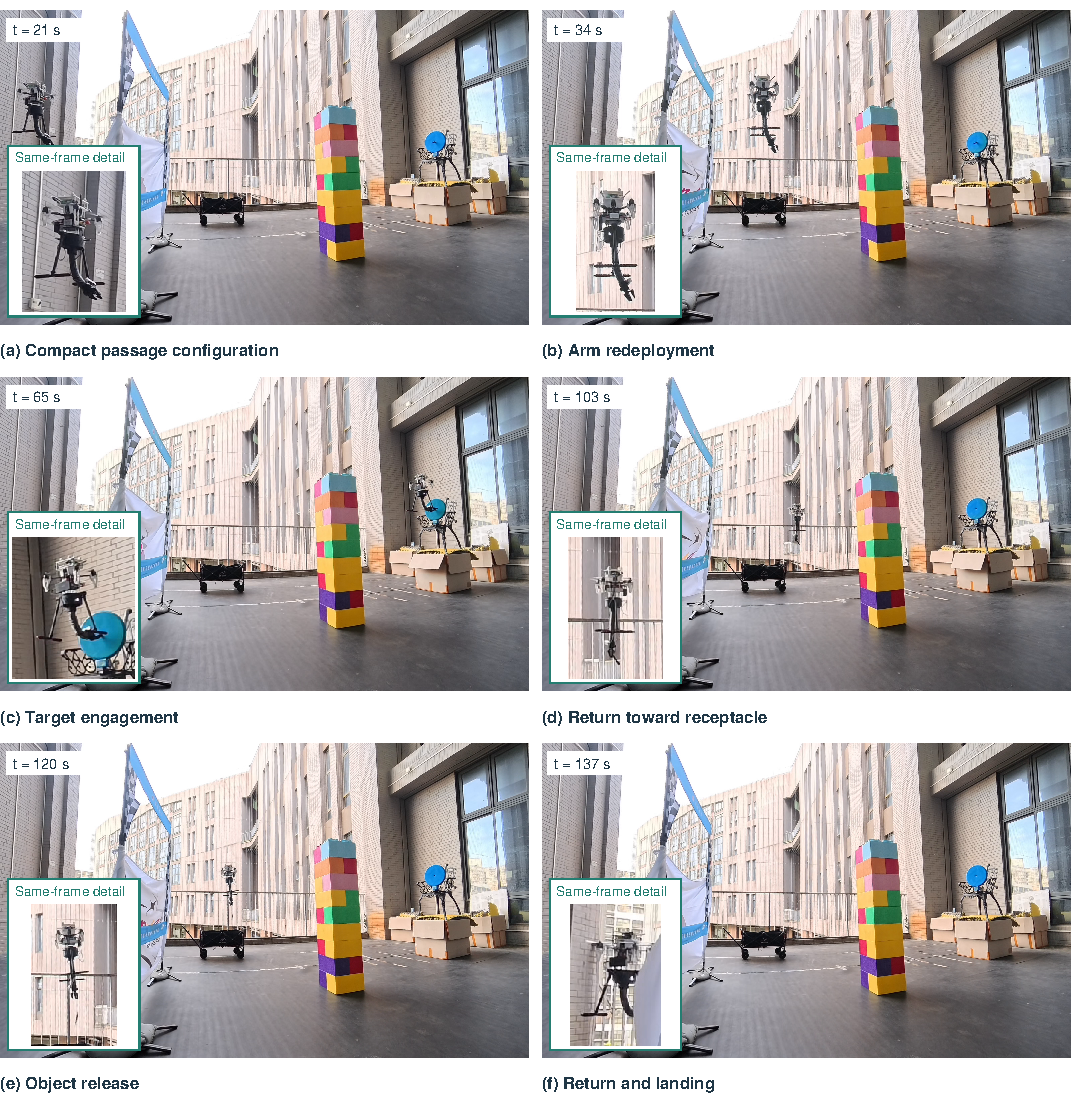
\includegraphics[width=\textwidth]{hardware_sequence_raw.pdf}
\caption{Physical demonstration of morphology-coordinated task execution. Frames sampled from one original video show (a) a compact configuration near the passage, (b) arm redeployment after passage, (c) target engagement, (d) return toward the receptacle, (e) object release, and (f) return and landing. Times refer to the source-video clock. All panels use the same scene crop; framed insets magnify the corresponding original frame. Robot and object shapes are preserved.}
\label{fig:hardware_sequence}
\end{figure*}

Figure~\ref{fig:hardware_sequence} presents the task sequence. The arm first adopts a compact configuration for passage and then redeploys to recover reach toward the target. Following target engagement, the vehicle returns toward the receptacle, releases the object, and returns to the landing area. The sequence illustrates the use of different continuum morphologies for transit and interaction within one task.

This physical sequence complements the simulation results at the level of task geometry: compact morphology accommodates the passage, whereas redeployment supports subsequent object interaction. The simulation comparisons quantify the planning mechanisms, and the hardware demonstration shows their physical task context.

% Draft-only reserved block. Populate it after the LiDAR-equipped re-flight.
\ifhardwareplaceholders
\begin{figure*}[!t]
\centering
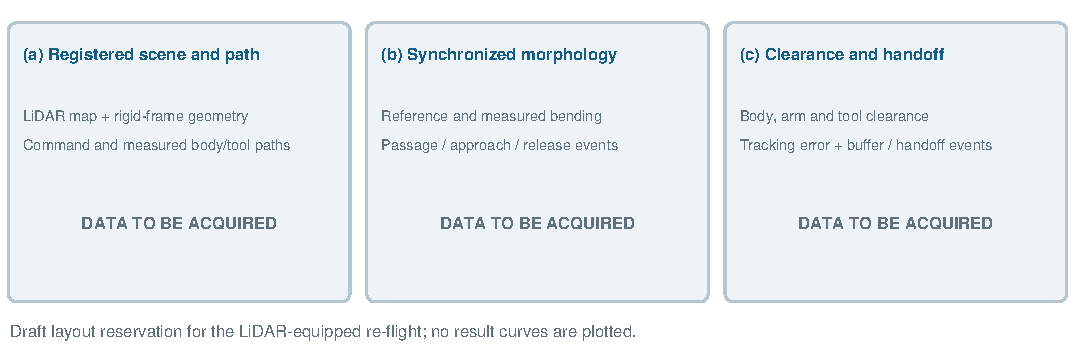
\includegraphics[width=\textwidth]{hardware_quantitative_slots.pdf}
\caption{Draft layout reserved for synchronized hardware evaluation: registered scene and trajectories, morphology tracking, and whole-body clearance with handoff events. Measurements will be inserted after the LiDAR-equipped re-flight.}
\label{fig:hardware_quantitative}
\end{figure*}
\begin{table}[t]
\centering
\caption{Draft hardware-evaluation fields for the planned re-flight.}
\label{tab:hardware_pending}
\small
\begin{tabular}{p{0.55\columnwidth}p{0.32\columnwidth}}
\toprule
Measure & Status\\\midrule
Attempts and completed tasks & To be acquired\\
Body / arm / tool minimum clearance & To be acquired\\
Position / bending tracking error & To be acquired\\
Planning latency and handoff events & To be acquired\\
Payload mass and release outcome & To be acquired\\\bottomrule
\end{tabular}
\end{table}
\fi
